\documentclass[runningheads]{llncs}

% ---------------------------------------------------------------
% Include basic ECCV package
 
\usepackage{eccv}

% OPTIONAL: Un-comment the following line for a version which is easier to read
% on small portrait-orientation screens (e.g., mobile phones, or beside other windows)
%\usepackage[mobile]{eccv}


% ---------------------------------------------------------------
% Other packages

% Commonly used abbreviations (\eg, \ie, \etc, \cf, \etal, etc.)
\usepackage{eccvabbrv}

% Include other packages here, before hyperref.
\usepackage{graphicx}
\usepackage{booktabs}
\usepackage{multirow}
\usepackage{algorithm}
\usepackage{algpseudocode}

% Keep absolute values aligned and append a compact relative delta on the right.
\newcommand{\scoredelta}[2]{\makebox[2.8em][r]{#1}\hspace{0.06em}{\scriptsize(#2)}}

% The "axessiblity" package can be found at: https://ctan.org/pkg/axessibility?lang=en
\usepackage[accsupp]{axessibility}  % Improves PDF readability for those with disabilities.


% ---------------------------------------------------------------
% Hyperref package

% It is strongly recommended to use hyperref, especially for the review version.
% Please disable hyperref *only* if you encounter grave issues.
% hyperref with option pagebackref eases the reviewers' job, but should be disabled for the final version.
%
% If you comment hyperref and then uncomment it, you should delete
% main.aux before re-running LaTeX.
% (Or just hit 'q' on the first LaTeX run, let it finish, and you
%  should be clear).

\usepackage{hyperref}

% Loosen float placement so figures land on or near their referring page.
\renewcommand{\topfraction}{0.9}
\renewcommand{\bottomfraction}{0.8}
\renewcommand{\textfraction}{0.07}
\renewcommand{\floatpagefraction}{0.75}
\setcounter{topnumber}{3}
\setcounter{bottomnumber}{2}
\setcounter{totalnumber}{5}

\begin{document}

% ---------------------------------------------------------------
\title{OREO: Fidelity Alignment in 3D Generation via On-the-fly Rendering-Editing Optimization}

\titlerunning{OREO: Fidelity Alignment in 3D Generation}

\author{Zhiyuan Ma\inst{1,2} \and
Wenbo Hu\inst{2}\textsuperscript{\dag} \and
Wang Zhao\inst{2} \and\\
Pengfei Wang\inst{1} \and
Ying Shan\inst{2} \and
Lei Zhang\inst{1}\textsuperscript{\dag}}

\authorrunning{Z. Ma et al.}
% First names are abbreviated in the running head.
% If there are more than two authors, 'et al.' is used.

\institute{The Hong Kong Polytechnic University
\and
Tencent ARC Lab}

\maketitle
\let\thefootnote\relax\footnotetext{\textsuperscript{\dag}Corresponding authors}


\begin{abstract}
  Despite recent advancements in 3D generation, models often struggle to produce assets with high visual fidelity.
  To bridge this gap, we propose OREO, an alignment framework that enhances the realism of 3D generators by leveraging rich 2D diffusion priors.
  Instead of relying on static datasets, OREO establishes a dynamic optimization loop that produces on-the-fly pseudo ground truths.
  At its core, OREO combines two components: (i) Reinforced Editing, which uses an image editor to refine rendered views of the 3D output, improving the visual fidelity of rendered views while preserving geometric structure; and (ii) Contrastive Distillation, which treats the edited views as positive and the original renderings as negative anchors, distilling the fidelity gap into the 3D generator via a latent contrastive objective.
  Experiments demonstrate that OREO effectively improves upon pre-trained baselines, producing 3D assets with enhanced visual realism.
  Our project page is at \url{https://theericma.github.io/oreo/}.
  \keywords{3D Generation  \and Alignment \and Image Diffusion Prior}
\end{abstract}

% NOTE: Terminology Distinction
% - Perceptual: Refers to high-level understanding, knowledge, and alignment (e.g., "perceptual priors", "perceptual misalignment").
% - Concept: Refers to specific objects, attributes, or content being generated/injected (e.g., "inject target concepts", "complex concepts").
% - Post-training Domain: Targets OOD domains (stylized/imaginative) uncovered by pre-training, bridging the gap via cross-modal transfer.

\section{Introduction}
\label{sec:intro}

\begin{figure}[!tbp]
  \centering
  \includegraphics[width=0.95\textwidth]{figures_final/OREO_teaser_v0.drawio.pdf}
  \caption{\textbf{Teaser.} To enhance visual fidelity of 3D generation, our framework first \textcolor{ForestGreen}{reinforces} rendered views via image editing, then distills the gap back to the training generator with a \textcolor{red}{latent contrastive} objective. Detailed workflow in Fig.~\ref{fig:pipeline}.}
  \label{fig:teaser}
  \vspace{-2mm}
\end{figure}

Recent 3D generators, such as Trellis~\cite{xiang2025structured} and the Hunyuan3D series~\cite{yang2024hunyuan3d,zhao2025hunyuan3d,hunyuan3d2025hunyuan3d,lai2025hunyuan3d2_5}, have greatly simplified the 3D content creation process.
However, despite their strong performance in geometry generation, achieving high visual fidelity remains challenging.
Generated assets often lack intricate textures and fine-grained details observed in real-world subjects.
This limitation largely stems from the scarcity of high-quality 3D data with diverse appearances, which pales in comparison to the vast visual knowledge encapsulated in billion-scale 2D imagery.
Consequently, 3D generative models may not fully capture the nuanced visual characteristics required for photorealistic rendering.

To bridge this gap, we propose to distill the rich visual priors of pre-trained 2D diffusion models into 3D generators.
These models encapsulate a deep understanding of visual fidelity and fine-grained details, far surpassing the scope of existing 3D datasets.
To this end, we introduce the On-the-fly Rendering Editing Optimization (OREO) framework, as illustrated in Fig.~\ref{fig:teaser}.
The core idea is to establish a dynamic alignment mechanism: instead of learning from static datasets, the generator improves by learning from pseudo ground truths generated on-the-fly.
Specifically, OREO implements a Render-Edit-Optimize loop, where the model renders views from its current output, receives corrective edits to enhance realism, and uses these refined views as supervision targets.

At the core of this loop is the Reinforced Editing algorithm, which generates high-quality supervision signals.
To ensure reliable guidance, Reinforced Editing prioritizes structure preservation, focusing on improving visual fidelity while maintaining the original spatial layout.
Inspired by recent inversion-free editing techniques, this approach mitigates the unwanted geometric deviations common in standard editing methods, ensuring that the generated pseudo-GTs remain geometrically aligned with the underlying 3D mesh.
To turn these refined targets into effective supervision, we propose Contrastive Distillation, which treats the edited view as a positive and the original rendering as a negative, and distills the fidelity gap into the 3D generator through a latent-space contrastive objective.
Experiments on the state-of-the-art Trellis model demonstrate that OREO effectively improves its performance, producing 3D assets with superior visual realism.
In summary, our contributions are as follows:
\begin{enumerate}\setlength{\itemsep}{0pt}
    \item We introduce OREO, a novel alignment framework that leverages pre-trained 2D diffusion priors to enhance the fidelity of 3D generators through an on-the-fly optimization loop with dynamic pseudo ground truths.
    \item At its core, we propose Reinforced Editing, an inversion-free algorithm that improves the visual fidelity of rendered views while preserving structure, coupled with Contrastive Distillation that turns the edited/original views into latent-space positive/negative anchors for effective generator post-training.
    \item We validate the effectiveness of OREO on state-of-the-art 3D generators. Results show that our method effectively improves visual fidelity while preserving geometric integrity.
\end{enumerate}

\section{Related Work}
\label{sec:related_work}

\noindent\textbf{Learning-based 3D Generation and Generator Post-training.}
Recent learning-based 3D generators synthesize assets feed-forward in latent spaces~\cite{xiang2025structured,zhao2025hunyuan3d,ye2025hi3dgen,li2025triposg,guo2025hyper3d,yushi2025gaussiananything,chen20253dtopia,lin2025diffsplat,li2025step1x,zhang2025bang,yang20264dvd,yang2026gencompositor,liang2026aligncvc,wang2026one2scene,liu2025mvboost}, but their reliance on synthetic data such as Objaverse~\cite{deitke2023objaverse} caps visual fidelity and texture detail.
OREO addresses this by transferring appearance priors from pretrained 2D diffusion models: it uses 2D image editing to lift rendered views into higher-fidelity, structure-preserving edited views, and treats the discrepancy as online supervision for post-training.

\noindent\textbf{2D Image Editing for Fidelity-Enhancing Supervision.}
Effective supervision requires edits that enhance fidelity while preserving viewpoint and structure.
Training-based image editors~\cite{brooks2023instructpix2pix,zhang2023magicbrush,sheynin2023emu,zhao2024ultraedit} inject appearance details but do not constrain viewpoint or layout, and inversion-based training-free methods~\cite{hertz2022prompt,mokady2023null} still suffer from inversion errors.
Inversion-free approaches~\cite{couairon2024flowedit,zhang2024rfinversion} instead couple source and target trajectories, avoiding inversion altogether; we build our Reinforced Editing on this line.

\noindent\textbf{2D Priors for 3D Editing and Generation.}
Although 2D priors have been explored for 3D editing and generation, existing methods do not directly meet the goal of post-training a feed-forward 3D generator.
On the one hand, 3D editing and geometry-conditioned editing methods, such as Instruct-NeRF2NeRF~\cite{haque2023instruct}, DreamEditor~\cite{zhuang2023dreameditor}, GaussianEditor~\cite{wang2024gaussianeditor}, DFFSplat~\cite{koh2026diffusion}, Image Sculpting~\cite{yenphraphai2024image}, MvDrag3D~\cite{chen2024mvdrag3d}, GeoDiffusion~\cite{chen2024geodiffusion}, and Omni-3DEdit~\cite{chen2026omni}, mainly target individual instances or scenes and typically rely on per-scene optimization, making it difficult to amortize the fidelity-enhancing prior into a generalizable 3D generator.
On the other hand, score-distillation methods such as DreamFusion~\cite{poole2022dreamfusion}, Magic3D~\cite{lin2023magic3d}, ProlificDreamer~\cite{wang2024prolificdreamer}, ScaleDreamer~\cite{ma2024scaledreamer}, Hybrid Fourier Score Distillation~\cite{yang2025hybrid}, and Progressive Rendering Distillation~\cite{ma2025progressive} are optimization-based text-to-3D methods whose input setting and inference pipeline differ from OREO's learning-based image-to-3D generator post-training, making them unsuitable for direct quantitative comparison.
DMD~\cite{yin2024onestep} is closer to a generator-learning paradigm and is therefore retained as a reasonable score-distillation ablation baseline; however, it still relies on implicit score-gradient supervision.
In contrast, OREO explicitly constructs high-fidelity, structure-aligned edited views as pseudo-GT and uses stable online supervision to post-train the 3D generator.

\section{Method}
\label{sec:method}

We present OREO, an alignment framework that enhances 3D visual fidelity via on-the-fly optimization.
An overview of the full pipeline is illustrated in Fig.~\ref{fig:pipeline}.
We leverage a pre-trained 2D editing model to construct pseudo ground truths on the fly, overcoming the inability to train without 3D ground-truth supervision.
Specifically, the generator performs on-policy sampling to obtain a denoised 3D asset at an intermediate step, which is then rendered into a 2D view from a sampled camera pose, as detailed in Sec.~\ref{sec:preliminaries}.
We then apply the image editing prior with our proposed Reinforced Editing in Sec.~\ref{sec:reinforced_editing} to enhance the view, improving visual fidelity while preserving structural consistency.
Finally, using the enhanced view as a dynamic supervision signal, the training method in Sec.~\ref{sec:optimization} distills the fidelity improvement back into the 3D generator.

\begin{figure}[!tbp]
  \centering
  \includegraphics[width=\textwidth,trim=60 0 60 0,clip]{figures_final/OREO_pipeline_v3.drawio.pdf}
  \caption{\textbf{Overview of OREO.} The training generator produces a 3D asset via on-policy ODE rollout that is rendered into a source view $x^{\texttt{src}}$. \textcolor{ForestGreen}{Reinforced Editing} turns $x^{\texttt{src}}$ into a high-fidelity target $x^{\texttt{tgt}}$, and \textcolor{red}{Contrastive Distillation} uses $(x^{\texttt{src}}, x^{\texttt{tgt}})$ as a negative/positive pair to supervise the generator in the latent space.}
  \label{fig:pipeline}
\end{figure}

\subsection{Problem Formulation}
\label{sec:problem_formulation}
Given a reference image $x^{\texttt{ref}}$, the 3D latent generator $G_\theta$ followed by a decoder $\mathcal{D}$ produces a 3D asset $\mathcal{A} = \mathcal{D}(G_\theta(x^{\texttt{ref}}))$.
A renderer $\mathcal{P}$ then projects $\mathcal{A}$ into a 2D view $x^{\texttt{src}} = \mathcal{P}(\mathcal{A}, \pi)$ under camera pose $\pi$.
In our training framework, a pre-trained 2D editor $\mathcal{E}_\phi$ then enhances this view into a higher-fidelity target $x^{\texttt{tgt}} = \mathcal{E}_\phi(x^{\texttt{src}}, x^{\texttt{ref}})$.
The generator is optimized by minimizing the discrepancy between the two:
\begin{equation}
\label{eq:task}
\theta^* = \arg\min_\theta \mathbb{E}_{x^{\texttt{ref}}, \pi}
\left[\mathcal{L}(x^{\texttt{src}}, x^{\texttt{tgt}})\right]
\end{equation}
where $\mathcal{L}$ is a supervision loss that encourages improved visual fidelity.


\subsection{Preliminaries}
\label{sec:preliminaries}
\textbf{Flow Matching Framework and Notation.}
Flow Matching models generation as an ODE process that transports Gaussian noise to the data distribution:
\begin{equation}
    dx_t = v(x_t; t, c) dt, \quad t \in [1, 0]
\end{equation}
where $x_t$ is the latent state at time $t$, and $c$ is the condition (e.g., text or image).
For better alignment to the condition $c$, Classifier-Free Guidance (CFG) is applied to the velocity field, using a null condition $\emptyset$ and a guidance scale $w$:
\begin{equation}
    \label{eq:cfg_guidance}
    v^{w}(x_t; t, c) = v(x_t; t, \emptyset) + w \cdot (v(x_t; t, c) - v(x_t; t, \emptyset))
\end{equation}
A key property used in our method is single-step estimation of the clean sample $\hat{x}_0$ from the intermediate state $x_t$:
\begin{equation}
    \label{eq:single_step_estimation}
    \hat{x}_0 = x_t - t \cdot v(x_t; t, c)
\end{equation}
To distinguish modalities, we use $z$ and $\theta$ for the 3D generator $v_\theta$, where $G_\theta$ denotes its ODE sampling process and the pre-trained frozen weights are denoted $v_{\theta_{pre}}$.
Similarly, we use $x$ and $\phi$ for the 2D editor $v_\phi$, where $\mathcal{E}_\phi$ denotes the multi-step editing process as described below.



\textbf{Inversion-Free Image Editing.}
We leverage FlowEdit~\cite{couairon2024flowedit}, an inversion-free method that modifies images by coupling source and target flow trajectories.
Starting from $x^{\texttt{src}}$, it iteratively updates the editing variable via $x^{\texttt{edit}} \leftarrow x^{\texttt{edit}} - \Delta t \cdot \tilde{v}$, where the differential velocity is defined as:
\begin{equation}
    \label{eq:flowedit_transition}
    \tilde{v} = v^{\texttt{tgt}}(x_t^{\texttt{tgt}}; t, c^{\texttt{tgt}}) - v^{\texttt{src}}(x_t^{\texttt{src}}; t, c^{\texttt{src}})
\end{equation}
where the \textbf{source branch} and the \textbf{target branch} is constructed as
\begin{equation}
    \label{eq:flowedit_states}
    x_t^{\texttt{src}} = (1-t)x^{\texttt{src}} + t\epsilon, \quad x_t^{\texttt{tgt}} = x^{\texttt{edit}} + (x_t^{\texttt{src}} - x^{\texttt{src}}), \quad \epsilon \sim \mathcal{N}(0, I).
\end{equation}
The editing process is performed over the last $N_e$ steps of the full $N$-step ODE schedule.
With integration step size $\Delta t = t_{i-1} - t_i$, $x^{\texttt{edit}}$ evolves into $x^{\texttt{tgt}}$, which transfers the image from being consistent with $c^{\texttt{src}}$ to following $c^{\texttt{tgt}}$ without the need for costly inversion that maps the image back to noise, thereby preserving structural fidelity.


\begin{algorithm}[t]
    \caption{Reinforced Editing}
    \label{alg:red}
    \begin{algorithmic}[1]
    \Require Rendered view $x^{\texttt{src}}$, Reference condition $c^{\texttt{ref}}$, Editor $\mathcal{E}_\phi$, Guidance scale $w$, Editing steps $N_e$, Total steps $N$
    \Ensure Pseudo-GT $x^{\texttt{tgt}}$
    \State Initialize $x^{\texttt{edit}} \leftarrow x^{\texttt{src}}$, Sample noise $\epsilon \sim \mathcal{N}(0, I)$
    \State Select time steps $\{t_i\}_{i=0}^{N_e}$ as the last $N_e$ steps from the full schedule of $N$ steps
    \For{$i = 0$ to $N_e-1$} \Comment{\texttt{FlowEdit: Backward Euler Integration}}
        \State $t \leftarrow t_i$, $\Delta t \leftarrow t_{i+1} - t_i$
        \State $x_t^{\texttt{src}} \leftarrow (1-t)x^{\texttt{src}} + t\epsilon$
        \State $x_t^{\texttt{tgt}} \leftarrow x^{\texttt{edit}} + (x_t^{\texttt{src}} - x^{\texttt{src}})$ \Comment{\texttt{Eq.~\ref{eq:flowedit_states}}}
        
        \Statex \texttt{// Reinforced Editing (Sec.~\ref{sec:reinforced_editing})}
        \State $\tilde{v} \leftarrow v_\phi^{w}(x_t^{\texttt{tgt}}; t, c^{\texttt{ref}}) - v_\phi(x_t^{\texttt{src}}; t, \emptyset)$ \Comment{\texttt{Eq.~\ref{eq:red_diff_velocity}}}
        \State $x^{\texttt{edit}} \leftarrow x^{\texttt{edit}} - \tilde{v} \Delta t$ \Comment{\texttt{FlowEdit: Euler Step}}
    
        \Statex \texttt{// Noise Update}
        \State $\epsilon \leftarrow \epsilon - (v_\phi(x_t^{\texttt{tgt}}; t, c^{\texttt{ref}}) - v_\phi(x_t^{\texttt{tgt}}; t, \emptyset)) \cdot (1-t)$ \Comment{\texttt{Eq.~\ref{eq:red_dynamic_noise}}}
    \EndFor
    \State \Return $x^{\texttt{tgt}} \leftarrow x^{\texttt{edit}}$
    \end{algorithmic}
    \end{algorithm}


\subsection{Constructing On-the-fly Pseudo-GTs via Reinforced Editing}
\label{sec:reinforced_editing}

A critical step in our pipeline is transforming the rendered view $x^{\texttt{src}}$ into a high-fidelity pseudo ground truth $x^{\texttt{tgt}}$.
Existing image editing models~\cite{wu2025qwen} can leverage their learned priors to make rendered views more realistic, but often alter the camera perspective or object pose, as analyzed in Sec.~\ref{sec:exp_feedback}.
We propose Reinforced Editing to enable structure-preserving enhancement on top of pre-trained editing models.
Different from the original FlowEdit~\cite{couairon2024flowedit} that transfers between separate conditions $c^{\texttt{src}}$ and $c^{\texttt{tgt}}$ in Eq.~\ref{eq:flowedit_transition}, our goal is to enhance the rendered view to better resemble a novel view of $x^{\texttt{ref}}$, where no independent $c^{\texttt{src}}$ exists.
We thus guide the target branch toward $c^{\texttt{ref}} = c^{\texttt{tgt}}$ and replace the source branch with an unconditional prediction:
\begin{equation}
    \label{eq:red_diff_velocity}
    \tilde{v} = v_\phi^{w}(x_t^{\texttt{tgt}}; t, c^{\texttt{ref}}) - v_\phi(x_t^{\texttt{src}}; t, \emptyset),
\end{equation}
where $v_\phi$ is the velocity field of the pre-trained 2D editor, $w$ is the classifier-free guidance scale~\cite{ho2021classifier}, and $c^{\texttt{ref}}$ encodes both the reference image $x^{\texttt{ref}}$ and a text prompt indicating a viewpoint change, as illustrated in Fig.~\ref{fig:pipeline}.

\textbf{Noise Update.}
The editing effect may be insufficient because the shared noise $\epsilon$ in Eq.~\ref{eq:flowedit_states} is randomly sampled in each iteration, whose stochasticity can weaken the editing strength~\cite{xie2026dnaedit}.
To address this, we dynamically update $\epsilon$ at each step by injecting the classifier-free guidance signal into the noise:
\begin{equation}
    \label{eq:red_dynamic_noise}
    \epsilon \leftarrow \epsilon - (v_\phi(x_t^{\texttt{tgt}}; t, c^{\texttt{ref}}) - v_\phi(x_t^{\texttt{tgt}}; t, \emptyset)) \cdot (1-t)
\end{equation}
This update aligns the noise with the conditional direction, strengthening the editing effect while preserving fine-grained structural details.
The complete procedure is summarized in Algorithm~\ref{alg:red}.


\begin{algorithm}[t]
    \caption{Closed-loop Optimization via Dynamic Pseudo-GTs}
    \label{alg:oreo}
    \begin{algorithmic}[1]
    \Require Generator $v_\theta$, frozen pretrained velocity $v_{\theta_{pre}}$, 2D editor $\mathcal{E}_\phi$, learning rate $\eta$
    \Ensure Optimized parameters $\theta^*$
    \While{not converged}
        \State Given reference image $x^{\texttt{ref}}$
        \State $z_0 = G_\theta(x^{\texttt{ref}})$ \Comment{\texttt{Rollout}: Generate clean latent}
        \State Sample camera pose $\pi$
        \State $x^{\texttt{src}} = \mathcal{P}(\mathcal{D}(z_0), \pi)$ \Comment{\texttt{Render}: Decode and project}
        \State Obtain $x^{\texttt{tgt}}$ via Algorithm~\ref{alg:red} from $x^{\texttt{src}}$ and $x^{\texttt{ref}}$ \Comment{\texttt{Reinforced Editing}}
        \State Sample $t \sim \mathcal{U}(0,1)$
        \State $z_t = (1-t)z_0 + t\epsilon,\ \epsilon \sim \mathcal{N}(0,I)$ \Comment{\texttt{Noise Injection}}
        \State Predict $\hat{z}_0$ from $z_t$ using $v_\theta$ \Comment{\texttt{Prediction}: Denoise latent, Eq.~\ref{eq:single_step_estimation}}
        \State $\hat{z}_t = (1-t)\hat{z}_0 + t\epsilon',\ \epsilon' \sim \mathcal{N}(0,I)$ \Comment{\texttt{Re-noise anchor prediction}}
        \State $z_0^{+} = \hat{z}_t - t \cdot v_{\theta_{pre}}(\hat{z}_t; t, x^{\texttt{tgt}})$ \Comment{\texttt{Positive}, Eq.~\ref{eq:contrast_pos_neg}}
        \State $z_0^{-} = \hat{z}_t - t \cdot v_{\theta_{pre}}(\hat{z}_t; t, x^{\texttt{src}})$ \Comment{\texttt{Negative}, Eq.~\ref{eq:contrast_pos_neg}}
        \State $\mathcal{L}_{contrast} = \| \hat{z}_0 - z_0^{+} \|^2 - \| \hat{z}_0 - z_0^{-} \|^2$ \Comment{\texttt{Latent contrastive loss}, Eq.~\ref{eq:contrast_loss}}
        \State $\mathcal{L}_{reg} = \| v_\theta(z_t) - v_{\theta_{pre}}(z_t) \|^2$ \Comment{\texttt{Regularization}}
        \State $\theta \leftarrow \theta - \eta \nabla_\theta (\mathcal{L}_{contrast} + \lambda \mathcal{L}_{reg})$ \Comment{\texttt{Update generator}}
    \EndWhile
    \end{algorithmic}
    \end{algorithm}
    


\subsection{Contrastive Distillation with Pseudo-GTs}
\label{sec:optimization}


To instantiate the abstract loss $\mathcal{L}$ in Eq.~\ref{eq:task} for the 3D latent generator $G_\theta$, we lift the supervision from the pixel space of $x^{\texttt{src}}, x^{\texttt{tgt}}$ into the latent space of the pretrained generator $v_{\theta_{pre}}$, and cast it as a contrastive objective: we treat the generator's predicted clean latent $\hat{z}_0$ as an \emph{anchor}, with $x^{\texttt{tgt}}$ inducing a positive and $x^{\texttt{src}}$ inducing a negative, pulling the anchor toward the positive while pushing it away from the negative. This closes the Render-Edit-Optimize loop.

\textbf{Per-Iteration Setup.}
Concretely, in each training iteration, given a reference image $x^{\texttt{ref}}$, we roll out a clean latent $z_0 = G_\theta(x^{\texttt{ref}})$ via ODE sampling.
We then sample a camera pose $\pi$ and render $x^{\texttt{src}} = \mathcal{P}(\mathcal{D}(z_0), \pi)$.
From it we obtain a pseudo-GT $x^{\texttt{tgt}}$ via Reinforced Editing in Algorithm~\ref{alg:red}.
Finally, we sample a timestep $t \sim \mathcal{U}(0,1)$, perturb the latent as $z_t = (1-t)z_0 + t\epsilon$ with $\epsilon \sim \mathcal{N}(0,I)$, and recover the single-step prediction
\begin{equation}
\hat{z}_0 = z_t - t \cdot v_\theta(z_t; t, x^{\texttt{ref}}),
\end{equation}
which serves as the anchor in our contrastive objective below.

\textbf{Latent-Space Contrastive Supervision.}
Inspired by~\cite{yu2026self}, we re-noise the anchor with a fresh draw $\epsilon' \sim \mathcal{N}(0,I)$ as $\hat{z}_t = (1-t)\hat{z}_0 + t\epsilon'$, and run the frozen pretrained generator in two passes that share $\hat{z}_t$ but differ in their visual condition,
\begin{equation}
\label{eq:contrast_pos_neg}
z_0^{+} = \hat{z}_t - t \cdot v_{\theta_{pre}}(\hat{z}_t; t, x^{\texttt{tgt}}),
\quad
z_0^{-} = \hat{z}_t - t \cdot v_{\theta_{pre}}(\hat{z}_t; t, x^{\texttt{src}}).
\end{equation}
Both $z_0^{+}$ and $z_0^{-}$ are detached from the computational graph and serve as the positive and the negative, respectively. Under $x^{\texttt{tgt}}$ the pretrained generator denoises toward the edited pseudo-GT, while under $x^{\texttt{src}}$ it denoises toward the un-edited rendering.
The contrastive objective then pulls the anchor $\hat{z}_0$ toward $z_0^{+}$ and pushes it away from $z_0^{-}$,
\begin{equation}
\label{eq:contrast_loss}
\mathcal{L}_{contrast} = \| \hat{z}_0 - z_0^{+} \|^2 - \| \hat{z}_0 - z_0^{-} \|^2.
\end{equation}
To preserve geometric stability, we further regularize the velocity field deviation from the pre-trained prior,
\begin{equation}
\mathcal{L}_{reg} = \| v_\theta(z_t) - v_{\theta_{pre}}(z_t) \|^2,
\end{equation}
giving the total objective $\mathcal{L}_{total} = \mathcal{L}_{contrast} + \lambda \mathcal{L}_{reg}$.
The overall training procedure is summarized in Algorithm~\ref{alg:oreo}.


\section{Experiments}
\label{sec:experiments}

\subsection{Experimental Setup}
\label{sec:exp_setup}

\textbf{Datasets.}
Existing 3D benchmarks such as Objaverse~\cite{deitke2023objaverse} subsets focus on everyday objects, where pre-trained baselines already do well and fidelity gaps stay hidden.
To cover the more complex needs of image-to-3D users, especially imaginative and diverse concept-design tasks, we curate a \textit{Conceptual Design Dataset} of 2{,}396 in-the-wild reference images under-served by existing 3D priors.
We hold out 100 references for evaluation and use the remaining 2{,}296 for training. OREO uses these images alone and requires no paired 3D ground truth.
Curation and filtering details are in the \emph{Supp.\ Material}.
For a general-distribution reference, we additionally evaluate on Google Scanned Objects (GSO)~\cite{downs2022google}.

\textbf{Implementation Details.}
We use Trellis~\cite{xiang2025structured} as the 3D backbone and Qwen-Image-Edit~\cite{wu2025qwen} for Reinforced Editing, whose hyper-parameters are given in Sec.~\ref{sec:exp_feedback}.
Training details are provided in the \emph{Supp.\ Material}.

\begin{figure*}[!tbp]
    \centering
    \includegraphics[width=\textwidth]{figures_final/OREO_Edit_Comparisonv2_cropped.pdf}
    \caption{\textbf{Qualitative comparison of 2D feedback sources.} An ideal $x^{\texttt{tgt}}$ keeps the viewpoint of $x^{\texttt{src}}$ but lifts its fidelity toward $x^{\texttt{ref}}$; we compare Reinforced Editing (Ours), NanoBanana Pro, and Qwen-Image-Edit. Details are discussed in Sec.~\ref{sec:exp_feedback}.}
    \label{fig:edit_comparison}
  \end{figure*}


\begin{table*}[!tbp]
    \centering
    \caption{\textbf{Quantitative comparison of 2D feedback sources.} We report CLIP and DINO similarity to the reference $x^{\texttt{ref}}$ for fidelity and to the source view $x^{\texttt{src}}$ for content preservation, together with Mask IoU for viewpoint consistency. Details are in Sec.~\ref{sec:exp_feedback}.}
    \label{tab:feedback_comparison}
    \setlength{\tabcolsep}{3pt}
    \resizebox{\textwidth}{!}{%
    \begin{tabular}{@{}lccccc@{}}
      \toprule
      \multirow{2}{*}{Method} & \multicolumn{2}{c}{w.r.t.\ $x^{\texttt{ref}}$} & \multicolumn{2}{c}{w.r.t.\ $x^{\texttt{src}}$} & \multirow{2}{*}{IoU $\uparrow$} \\
      \cmidrule(lr){2-3}\cmidrule(lr){4-5}
      & CLIP Sim. $\uparrow$ & DINO Sim. $\uparrow$ & CLIP Sim. $\uparrow$ & DINO Sim. $\uparrow$ & \\
      \midrule
      Unedited & 0.7613 & 0.7915 & N/A & N/A & N/A \\
      \cmidrule(lr){1-6}
      NanoBanana Pro & \textbf{0.8803} & \textbf{0.9001} & 0.8199 & 0.8404 & 0.6830 \\
      Qwen-Edit (Orig.) & 0.7753 & 0.8269 & 0.7882 & 0.8084 & 0.6374 \\
      \midrule
      Ours & \scoredelta{0.7992}{+0.0379} & \scoredelta{0.8214}{+0.0299} & \textbf{0.8833} & \textbf{0.9099} & \textbf{0.9520} \\
      \bottomrule
    \end{tabular}}
  \end{table*}

  
\subsection{Validating the Editing Feedback}
\label{sec:exp_feedback}

The 3D generator is supervised by pseudo-GTs from a 2D editor, so the quality of these edits directly bounds what the 3D loop can achieve. 
We therefore first evaluate the editor's feedback at the 2D level, before 3D training.

\textbf{Evaluation Protocol.}
For each reference in the Conceptual Design Dataset, we generate a 3D asset with Trellis and render 5 views at azimuths $-90^\circ$, $-45^\circ$, $0^\circ$, $45^\circ$, and $90^\circ$ as source views $x^{\texttt{src}}$.
To evaluate the editing performance, we adopt three metrics.
To measure the multi-view fidelity improvement, we compute the CLIP-ViT-L/14~\cite{radford2021learning} and DINOv3-ViT-L/16~\cite{simeoni2025dinov3} embedding similarity of each rendered view to the reference $x^{\texttt{ref}}$, and report the mean over the 5 views before and after editing. To check content preservation, we additionally report the similarity to $x^{\texttt{src}}$.
Besides, to quantify the consistency of object pose, we use Mask IoU, with foreground masks extracted by U$^2$-Net~\cite{qin2020u2} as in Trellis.

\textbf{Compared Methods.}
We compare our Reinforced Editing (RE) against the original Qwen-Image-Edit~\cite{wu2025qwen} pipeline and NanoBanana Pro.
The setup for the compared methods is provided in the \emph{Supp.\ Material}.



\textbf{Qualitative Analysis.}
Fig.~\ref{fig:edit_comparison} visualizes the feedback quality. A critical challenge is maintaining both the camera perspective and content fidelity of the source view $x^{\texttt{src}}$.
NanoBanana Pro primarily fails at controlling the viewpoint: when $x^{\texttt{src}}$ differs substantially in viewpoint from $x^{\texttt{ref}}$, it tends to abandon the $x^{\texttt{src}}$ viewpoint and revert to $x^{\texttt{ref}}$.
For instance, in row 1, $x^{\texttt{src}}$ shows the orc warrior from a side view, yet NanoBanana Pro's output snaps back to a frontal view nearly identical to $x^{\texttt{ref}}$.
Even when the viewpoint is roughly preserved, it is not faithful to the local content of the source view, e.g., the mage's cape in row 2 is altered.
In contrast, Reinforced Editing injects high-fidelity textures while strictly adhering to the source perspective and content layout, ensuring geometrically aligned supervision.
Qwen-Image-Edit fails at the pose level in an even more pronounced way: the orc warrior's hand pose is altered in row 1, the mage collapses into a tilted, falling posture in row 2, and the cowgirl in row 5 is cropped from a full-body figure into a half-body portrait. 
It also drifts on the background, which is occasionally washed to a plain gray tone.

\textbf{Quantitative Results.}
As shown in Table~\ref{tab:feedback_comparison}, the \textit{Unedited} row represents the raw rendered view $x^{\texttt{src}}$, quantifying its initial alignment with the reference $x^{\texttt{ref}}$.
Baseline editors can achieve high similarity to $x^{\texttt{ref}}$ but deviate substantially from $x^{\texttt{src}}$, which is evidenced by their low Mask IoU.
In contrast, RE maintains high similarity to $x^{\texttt{src}}$ while still improving semantic fidelity.



\textbf{Ablation Study on RE Parameters.}
We further study two key hyper-parameters of RE: the editing ratio $N_e/N$ and the absolute editing steps $N_e$, as discussed in Sec.~\ref{sec:reinforced_editing}.
As shown in Fig.~\ref{fig:ablation_ratio_steps}(a) and Fig.~\ref{fig:ablation_vis}(a), a low ratio of $0.25$ barely edits the source view: the mecha warrior in row 1 and the king in row 2 remain almost identical to $x^{\texttt{src}}$, with limited detail enhancement. 
Conversely, a full ratio of $1.0$ causes severe deviations from the source view; the mecha warrior is rendered at a shrunken scale with an altered pose, and the king loses part of its cape and body, leading to identity mismatch. 
In contrast, a ratio of $0.75$ improves texture fidelity while preserving the original silhouette and viewpoint. 
This is corroborated by Fig.~\ref{fig:ablation_ratio_steps}(a): CLIP and DINO similarity rise sharply from ratio $0.25$ to $0.75$, and then degrade markedly at ratio $1.0$.
Fig.~\ref{fig:ablation_ratio_steps}(b) shows that the primary gain concentrates between $6$ and $9$ steps, where CLIP and DINO similarity rise most steeply. 
Beyond $9$ steps the curves quickly flatten: the semantic gains from $15$ and $30$ steps are marginal, while Mask IoU keeps dropping as extra editing further deviates from $x^{\texttt{src}}$. 
Fig.~\ref{fig:ablation_vis}(b) visually confirms this saturation on facial details: at $9$ steps the two female characters already exhibit sharp facial features, such as clearly resolved eyes and skin shading; increasing steps to $15$ or $30$ yields fewer perceptible improvements in the face regions.
Therefore, we adopt $N_e=9$, $N=12$ in all subsequent 3D experiments for a better quality-efficiency balance.

\begin{figure}[!tbp]
  \centering
  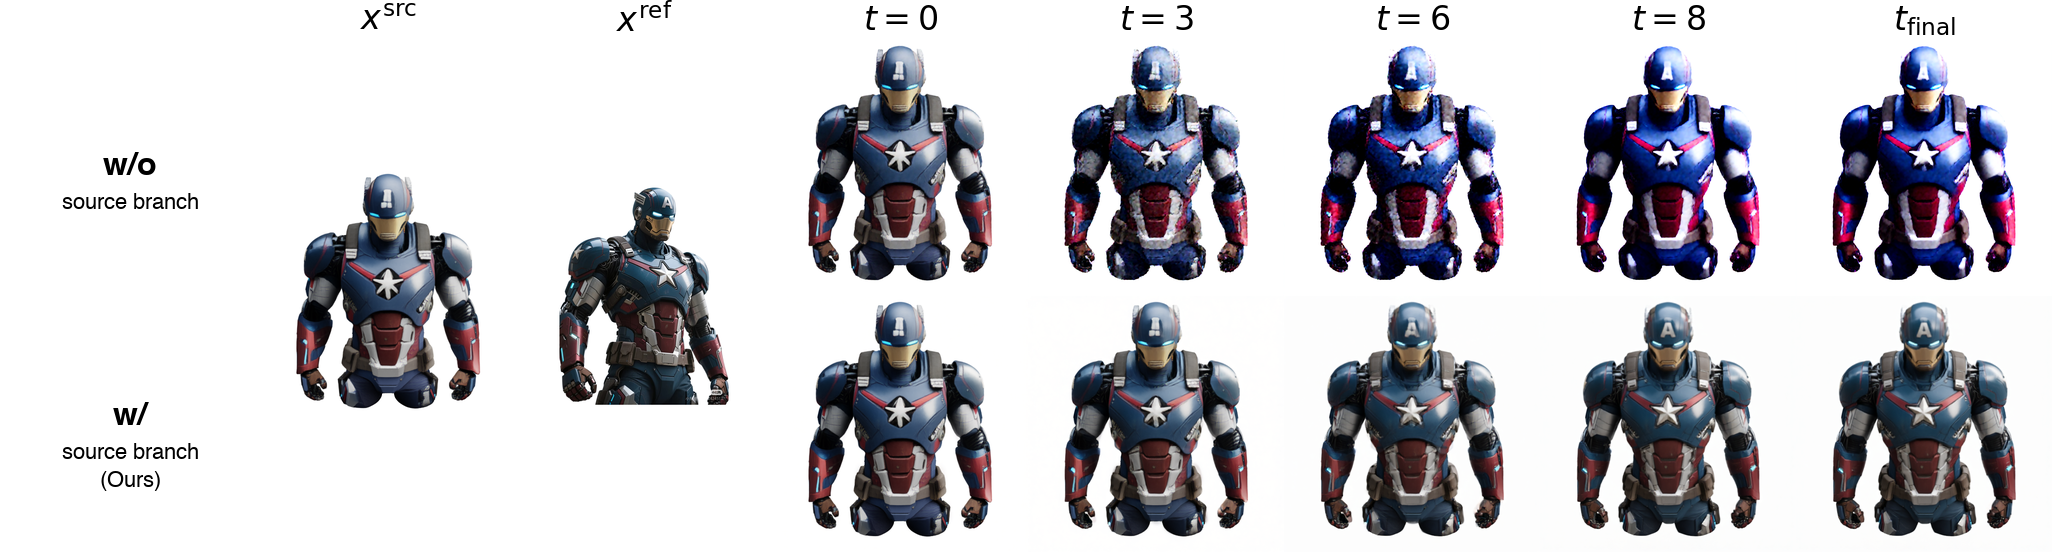
\includegraphics[width=\linewidth]{figures_rebuttal/comparison_grid.png}
  \caption{\textbf{Editing trajectories with and without the source branch.} Removing the source branch (top) leads to progressive color over-saturation and structural drift; keeping it (bottom, Ours) stabilizes the trajectory. Details in Sec.~\ref{sec:exp_feedback}.}
  \label{fig:neg_src_guidance}
\end{figure}

\textbf{Ablation Study on RE Components.}
RE builds on two key components, the source branch in Eq.~\ref{eq:red_diff_velocity} and the dynamic noise update in Eq.~\ref{eq:red_dynamic_noise}, and we ablate each in turn to see how much it contributes.
Without the source branch, only the target-conditioned velocity is used, and the trajectory drifts away from $x^{\texttt{src}}$: Fig.~\ref{fig:neg_src_guidance} shows the resulting color over-saturation and structural degradation, and Table~\ref{tab:ablation_components} reports negative $\Delta$CLIP and $\Delta$DINO, meaning the edited output is even less faithful to $x^{\texttt{ref}}$ than the unedited source.
Without the noise update, the per-step $\epsilon$ is resampled at random and no longer aligned with the conditional CFG direction, diluting the edit signal in the target--unconditional delta. Table~\ref{tab:ablation_components} shows $\Delta$CLIP and  $\Delta$DINO dropping to nearly zero, so the edit is applied but barely takes effect.
We evaluate whether these 2D-level benefits transfer to the downstream 3D generator in the next section.

\begin{table}[!tbp]
  \centering
  \caption{\textbf{Ablation on key components of Reinforced Editing.} We report $\Delta$CLIP and $\Delta$DINO, defined as the change in CLIP/DINO similarity to $x^{\texttt{ref}}$ before and after editing; higher is better. Details are in Sec.~\ref{sec:exp_feedback}.}
  \label{tab:ablation_components}
  \begin{tabular}{@{}lcc@{}}
    \toprule
    Variant & $\Delta$CLIP Sim. $\uparrow$ & $\Delta$DINO Sim. $\uparrow$ \\
    \midrule
    Full (Ours) & \textbf{+0.0379} & \textbf{+0.0299} \\
    w/o Source Branch & $-0.0523$ & $-0.0497$ \\
    w/o Noise Update & $-0.0001$ & $+0.0089$ \\
    \bottomrule
  \end{tabular}
\end{table}


\begin{figure*}[!tbp]
  \centering
  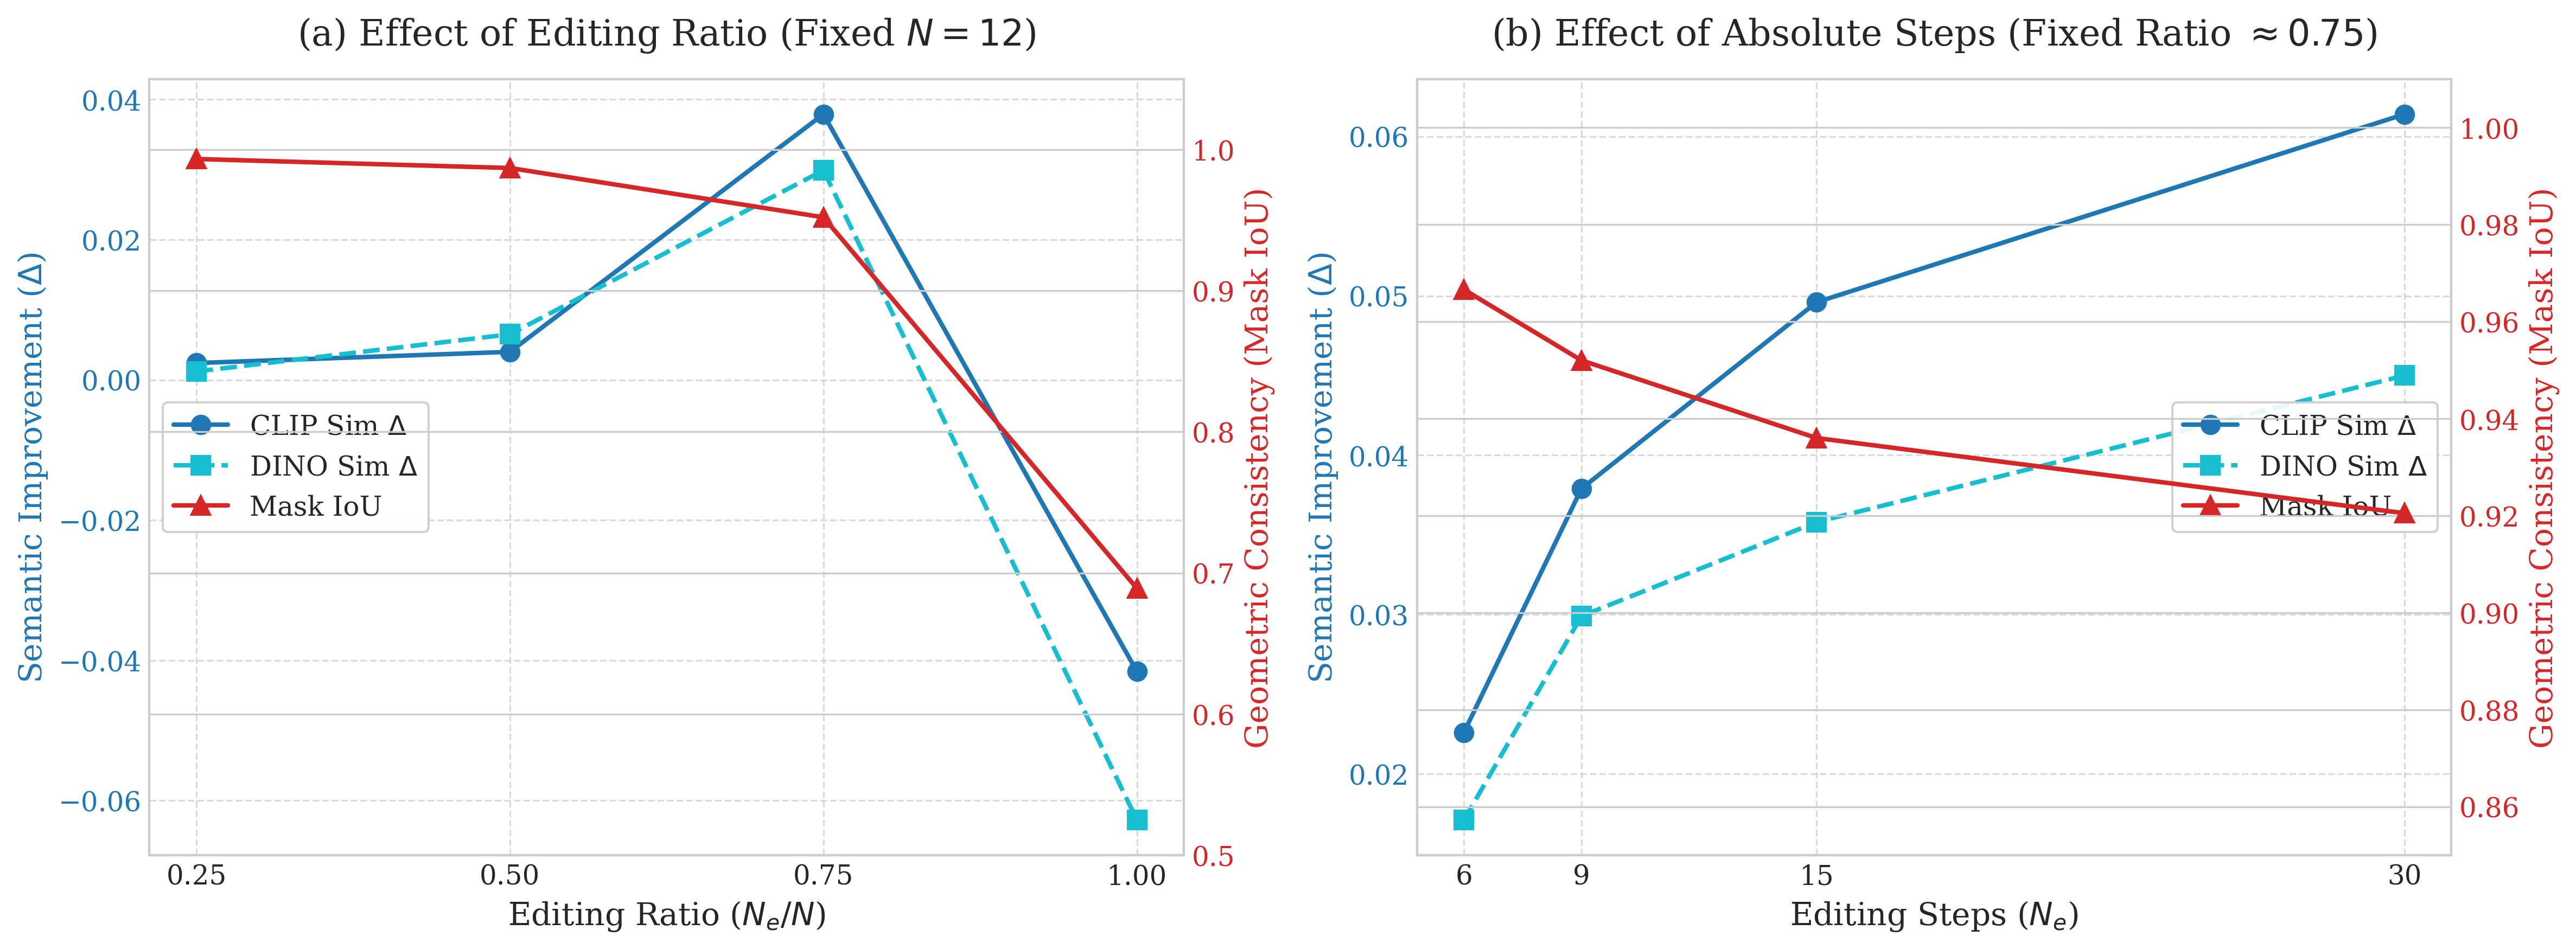
\includegraphics[width=\textwidth]{figures_final/ablation_ratio_steps.png}
  \caption{Sensitivity Analysis of RE Parameters. (a) \textbf{Effect of Editing Ratio ($N_e/N$)}: A ratio of 0.75 yields the best trade-off between semantic improvement (CLIP/DINO $\Delta$) and structural consistency (Mask IoU). (b) \textbf{Effect of Editing Steps ($N_e$)}: Under a fixed ratio ($\approx 0.75$), fewer steps (e.g., 9) achieve comparable performance to more expensive settings (e.g., 30) with significantly lower cost.}
  \label{fig:ablation_ratio_steps}
\end{figure*}

\begin{figure*}[!tbp]
  \centering
  \begin{subfigure}[b]{\textwidth}
    \centering
    \includegraphics[width=\textwidth]{figures_final/OREO_Ratiov2.pdf}
    \caption{Effect of Editing Ratio ($N_e/N$)}
  \end{subfigure}
  \par\smallskip
  \begin{subfigure}[b]{\textwidth}
    \centering
    \includegraphics[width=\textwidth]{figures_final/OREO_Stepsv2.pdf}
    \caption{Effect of Editing Steps ($N_e$)}
  \end{subfigure}
  \caption{Qualitative ablation study on RE parameters. (a) \textbf{Editing Ratio}: A low ratio (e.g., 0.25) limits editing capability, while a full ratio (1.0) destroys the original structure. Our choice of 0.75 strikes a balance. (b) \textbf{Editing Steps}: Increasing steps from 9 to 30 yields negligible visual improvement, confirming the efficiency of our setting.}
  \label{fig:ablation_vis}
\end{figure*}

\subsection{Main Results}
\label{sec:exp_main}

\textbf{Experimental Setup.}
We evaluate the 3D generation quality of Trellis distilled with OREO. 
As baselines, we compare against the pre-trained Trellis and Photo3D, a related post-training work built on the same Trellis backbone. 
Following the protocol in Sec.~\ref{sec:exp_feedback}, we render 5 views at azimuths $-90^\circ, -45^\circ, 0^\circ, 45^\circ, 90^\circ$ for each reference and report CLIP-ViT-L/14~\cite{radford2021learning} and DINOv3-ViT-L/16~\cite{simeoni2025dinov3} embedding similarity to the reference $x^{\texttt{ref}}$, averaged over the 5 views. 
In addition to our proposed Conceptual Design Dataset, which targets imaginative and out-of-distribution references, we further validate on GSO~\cite{downs2022google}, an in-distribution benchmark of common real-world objects, to verify that OREO does not compromise generation quality on the pre-trained model's original distribution.

\textbf{Quantitative and Qualitative Evaluation.}
Table~\ref{tab:main_results} summarizes the quantitative comparison. OREO achieves clear gains in CLIP and DINO similarity on the Conceptual Design Dataset, our target imaginative distribution. In contrast, the improvement on the in-distribution GSO benchmark is marginal, indicating that OREO's fidelity gain is targeted: on distributions that are not part of the training references, OREO preserves the pre-trained model's original quality rather than compromising it.
Fig.~\ref{fig:qualitative_comparison} shows the visual comparison. Compared with the pre-trained Trellis and Photo3D, OREO recovers finer appearance details while preserving the geometric structure and identity cues of $x^{\texttt{ref}}$. For example, OREO reconstructs the eye and spotted feather patterns on the parrot, the twisted tree trunk shape in the courtyard, and more consistent back-view colors on the minotaur.

\textbf{User Preference Study.}
To complement the automatic metrics, we further conduct a user preference study on the same held-out Conceptual Design Dataset, in which participants compare multi-view renderings from Pretrained Trellis, Photo3D, and OREO under blinded conditions.
OREO obtains the highest preference ratio, indicating that human evaluators more frequently favor its balance between reference fidelity, fine-grained detail, and multi-view consistency.
Full protocols and results are in the \emph{Supp.\ Material}.

\begin{table}[!tbp]
  \centering
  \caption{\textbf{Main quantitative comparison of 3D generation.} We report CLIP and DINO similarity to the reference $x^{\texttt{ref}}$ on the Conceptual Design Dataset and GSO. Details are in Sec.~\ref{sec:exp_main}.}
  \label{tab:main_results}
  \begin{tabular}{@{}lcccc@{}}
    \toprule
    \multirow{2}{*}{Method} & \multicolumn{2}{c}{Conceptual Design} & \multicolumn{2}{c}{GSO} \\
    \cmidrule(lr){2-3}\cmidrule(lr){4-5}
     & CLIP Sim. $\uparrow$ & DINO Sim. $\uparrow$ & CLIP Sim. $\uparrow$ & DINO Sim. $\uparrow$ \\
    \midrule
    Trellis & 0.7613 & 0.7916 & 0.7722 & 0.7022 \\
    Photo3D & 0.7380 & 0.7837 & 0.7512 & 0.7034 \\
    OREO (Ours) & \textbf{0.7834} & \textbf{0.8065} & \textbf{0.7764} & \textbf{0.7069} \\
    \bottomrule
  \end{tabular}
\end{table}
% \begin{itemize}
%     \item \textbf{Conceptual Alignment}: The higher CLIP score shows that OREO more effectively transfers concept cues from the edited pseudo-GTs to the 3D generator, consistent with the improved feedback quality observed in Section~\ref{sec:exp_feedback}.
%     \item \textbf{Structural Consistency}: The gain in DINO score suggests that OREO enhances texture and appearance details without sacrificing global structure, matching our design goal of realism enhancement under geometry preservation.
%     \item \textbf{Overall Effect}: These quantitative gains align with the qualitative comparisons in Fig.~\ref{fig:qualitative_comparison}, where OREO produces clearer details and more coherent multi-view results than the baseline.
% \end{itemize}
% \begin{itemize}
%     \item \textbf{Geometric Repair}: In the case of "Cyberpunk style mechanical prosthetic limbs", the original Trellis often generated blurred structures, while OREO successfully restored clear joint and pipeline details.
%     \item \textbf{Texture Enhancement}: For "Magic book with glowing runes", the textures generated by OREO were not only clearer but also had lighting effects more consistent with the prompt description, eliminating the oversaturation problem common in SDS.
%     \item \textbf{Multi-view Consistency}: Although FlowEdit guides on a single view, thanks to the inherent consistency of the 3D generator, the assets generated by OREO maintained structural coherence across all views, without obvious Janus problems.
% \end{itemize}

\begin{figure*}[!tbp]
  \centering
  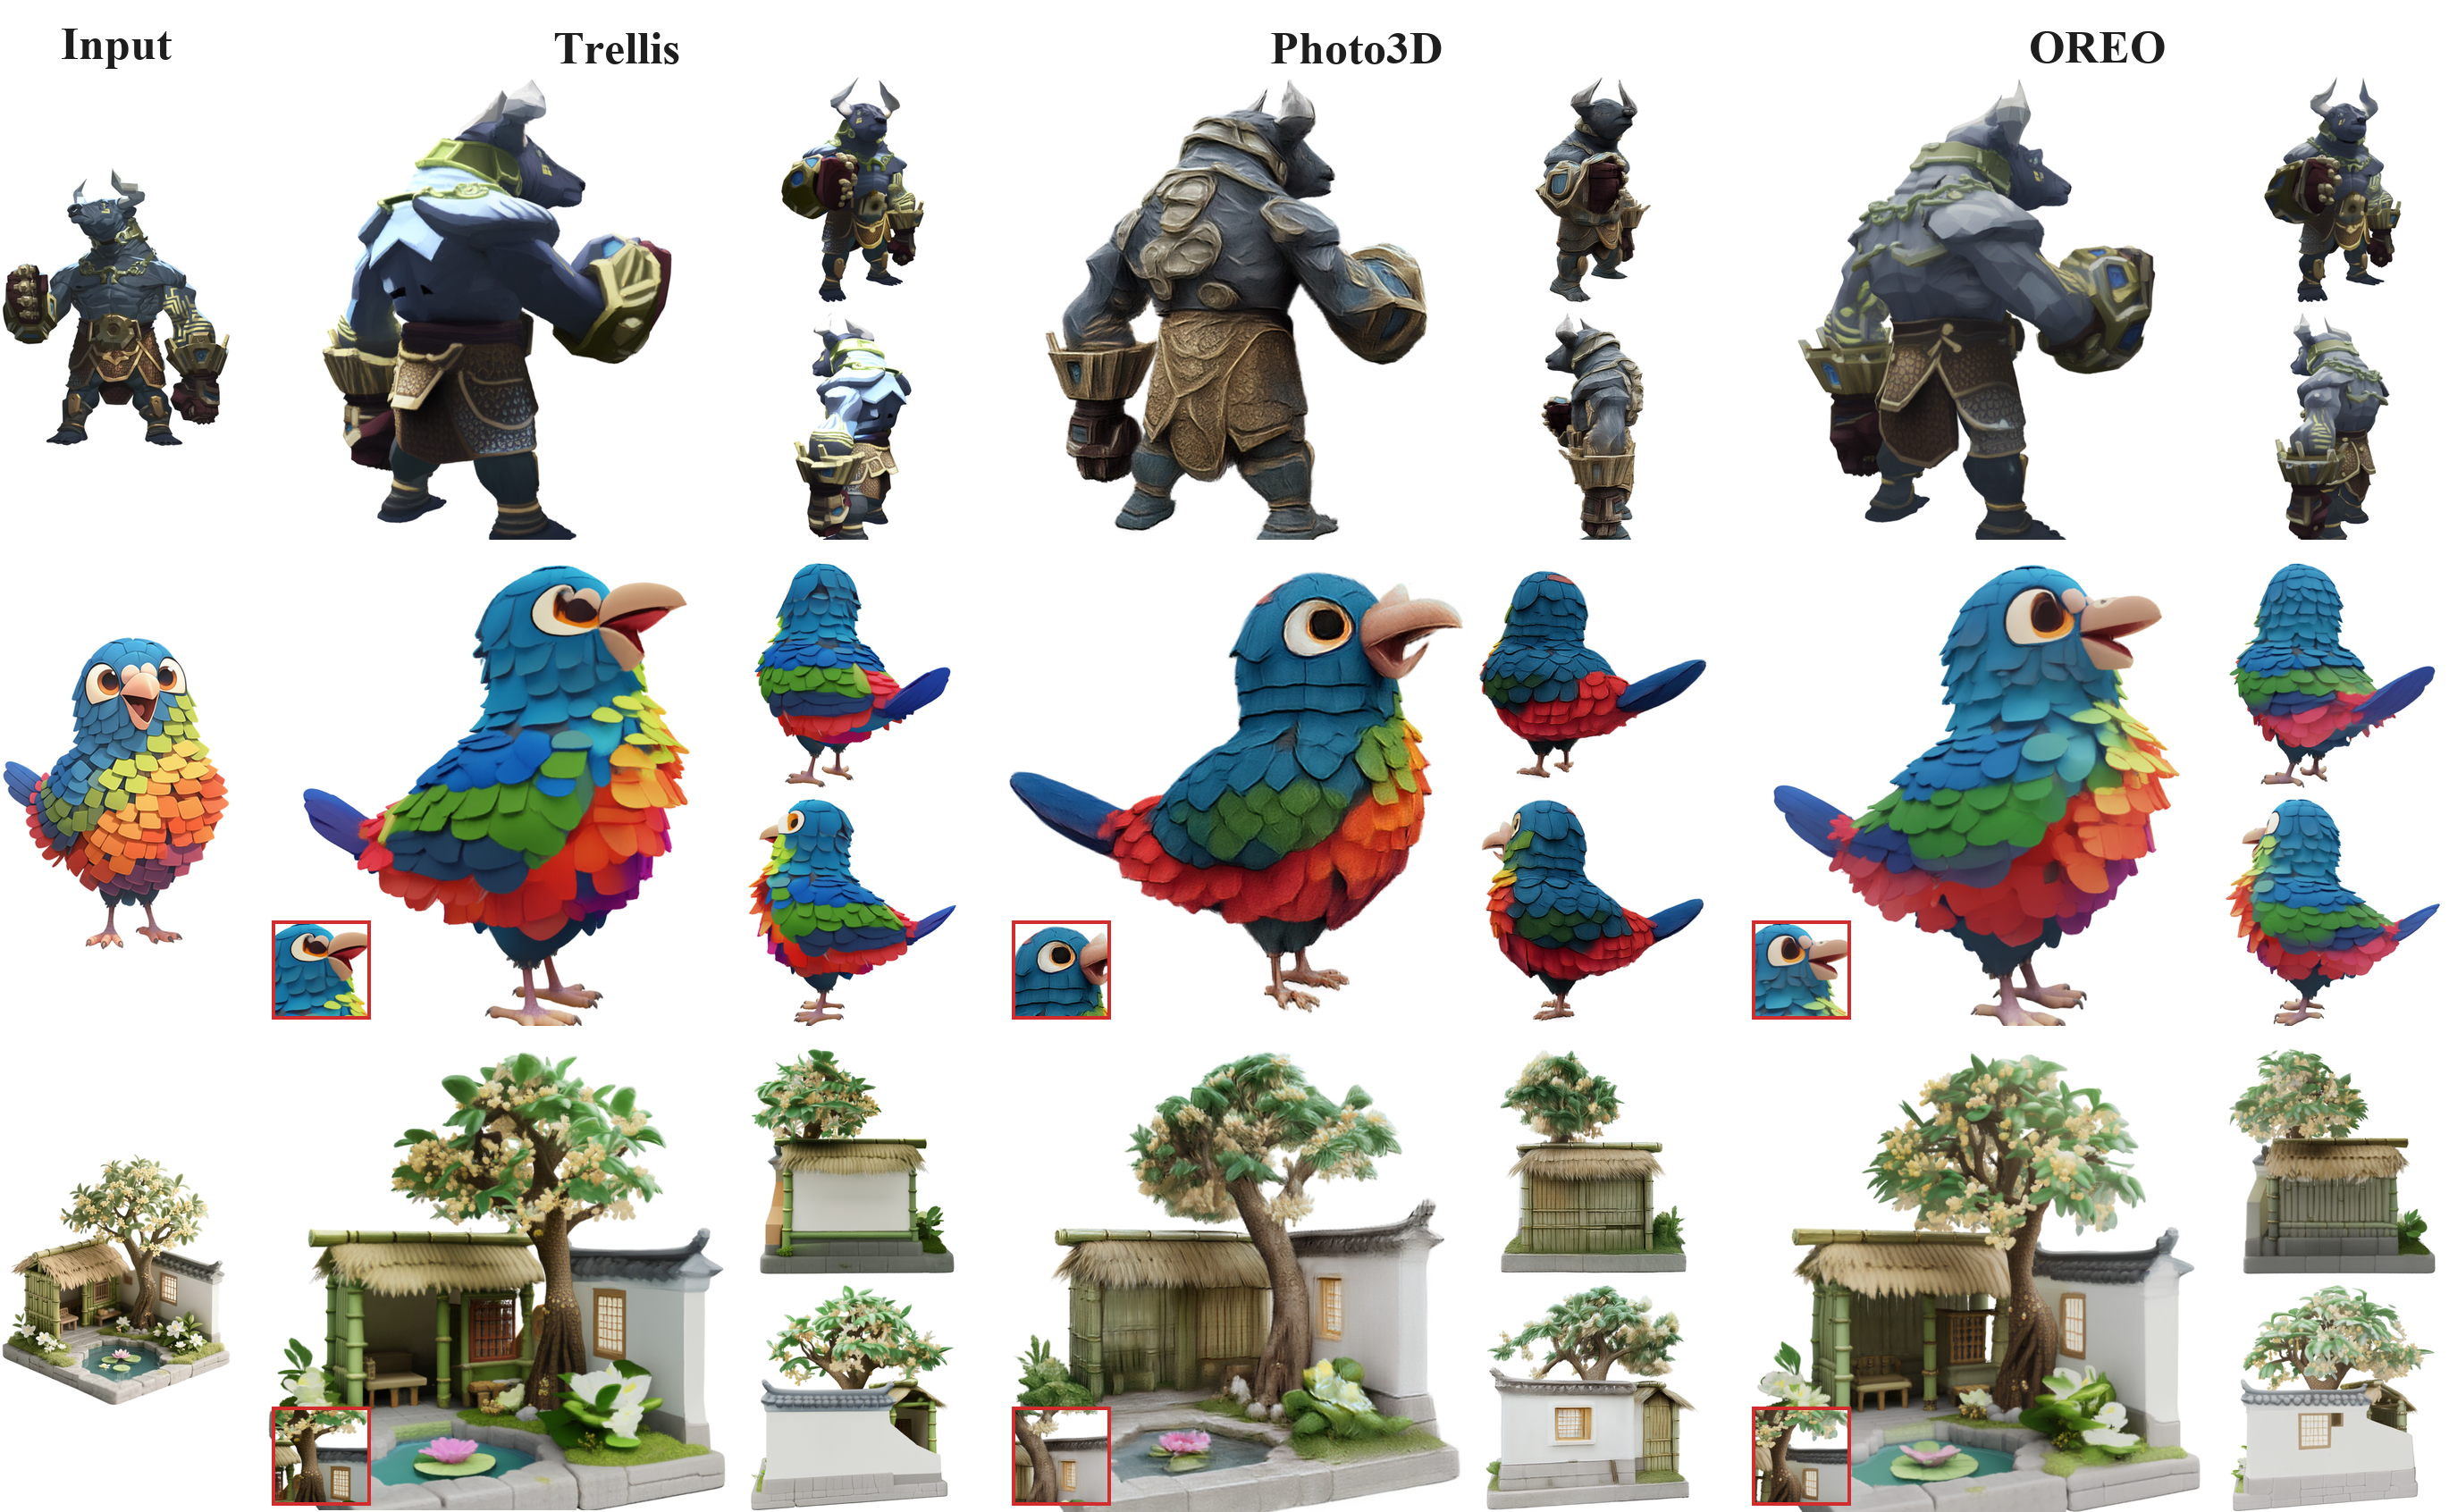
\includegraphics[width=\textwidth]{figures_final/mv_comparison_final.png}
  \caption{\textbf{Main qualitative comparison of 3D generation.} OREO delivers higher multi-view visual fidelity than Trellis and Photo3D. Details are in Sec.~\ref{sec:exp_main}.}
  \label{fig:qualitative_comparison}
\end{figure*}

\subsection{Ablation Study and Analysis}
\label{sec:exp_ablation}

Full OREO's training scheme rests on three designs. First, the rollout is \emph{on-policy}: the anchor $\hat{z}_0$ is derived from the training generator's own current output $G_\theta(x^{\texttt{ref}})$. Second, supervision is applied in the latent space via a contrastive objective, bypassing the differentiable renderer. Third, the contrastive target is built from an explicit multi-step pseudo-GT produced by Reinforced Editing. We ablate them with three variants: \emph{w/ Off-policy Rollout} freezes the rollout to $G_{\theta_{pre}}(x^{\texttt{ref}})$; \emph{w/ Pixel-MSE Supervision} regresses in pixel space; \emph{w/ DMD} drops the explicit target and instead uses a single-step score-distillation gradient. Table~\ref{tab:ablation_quantitative} shows all three fall below the pretrained Trellis baseline while Full OREO improves over it.

\begin{figure*}[!tbp]
  \centering
  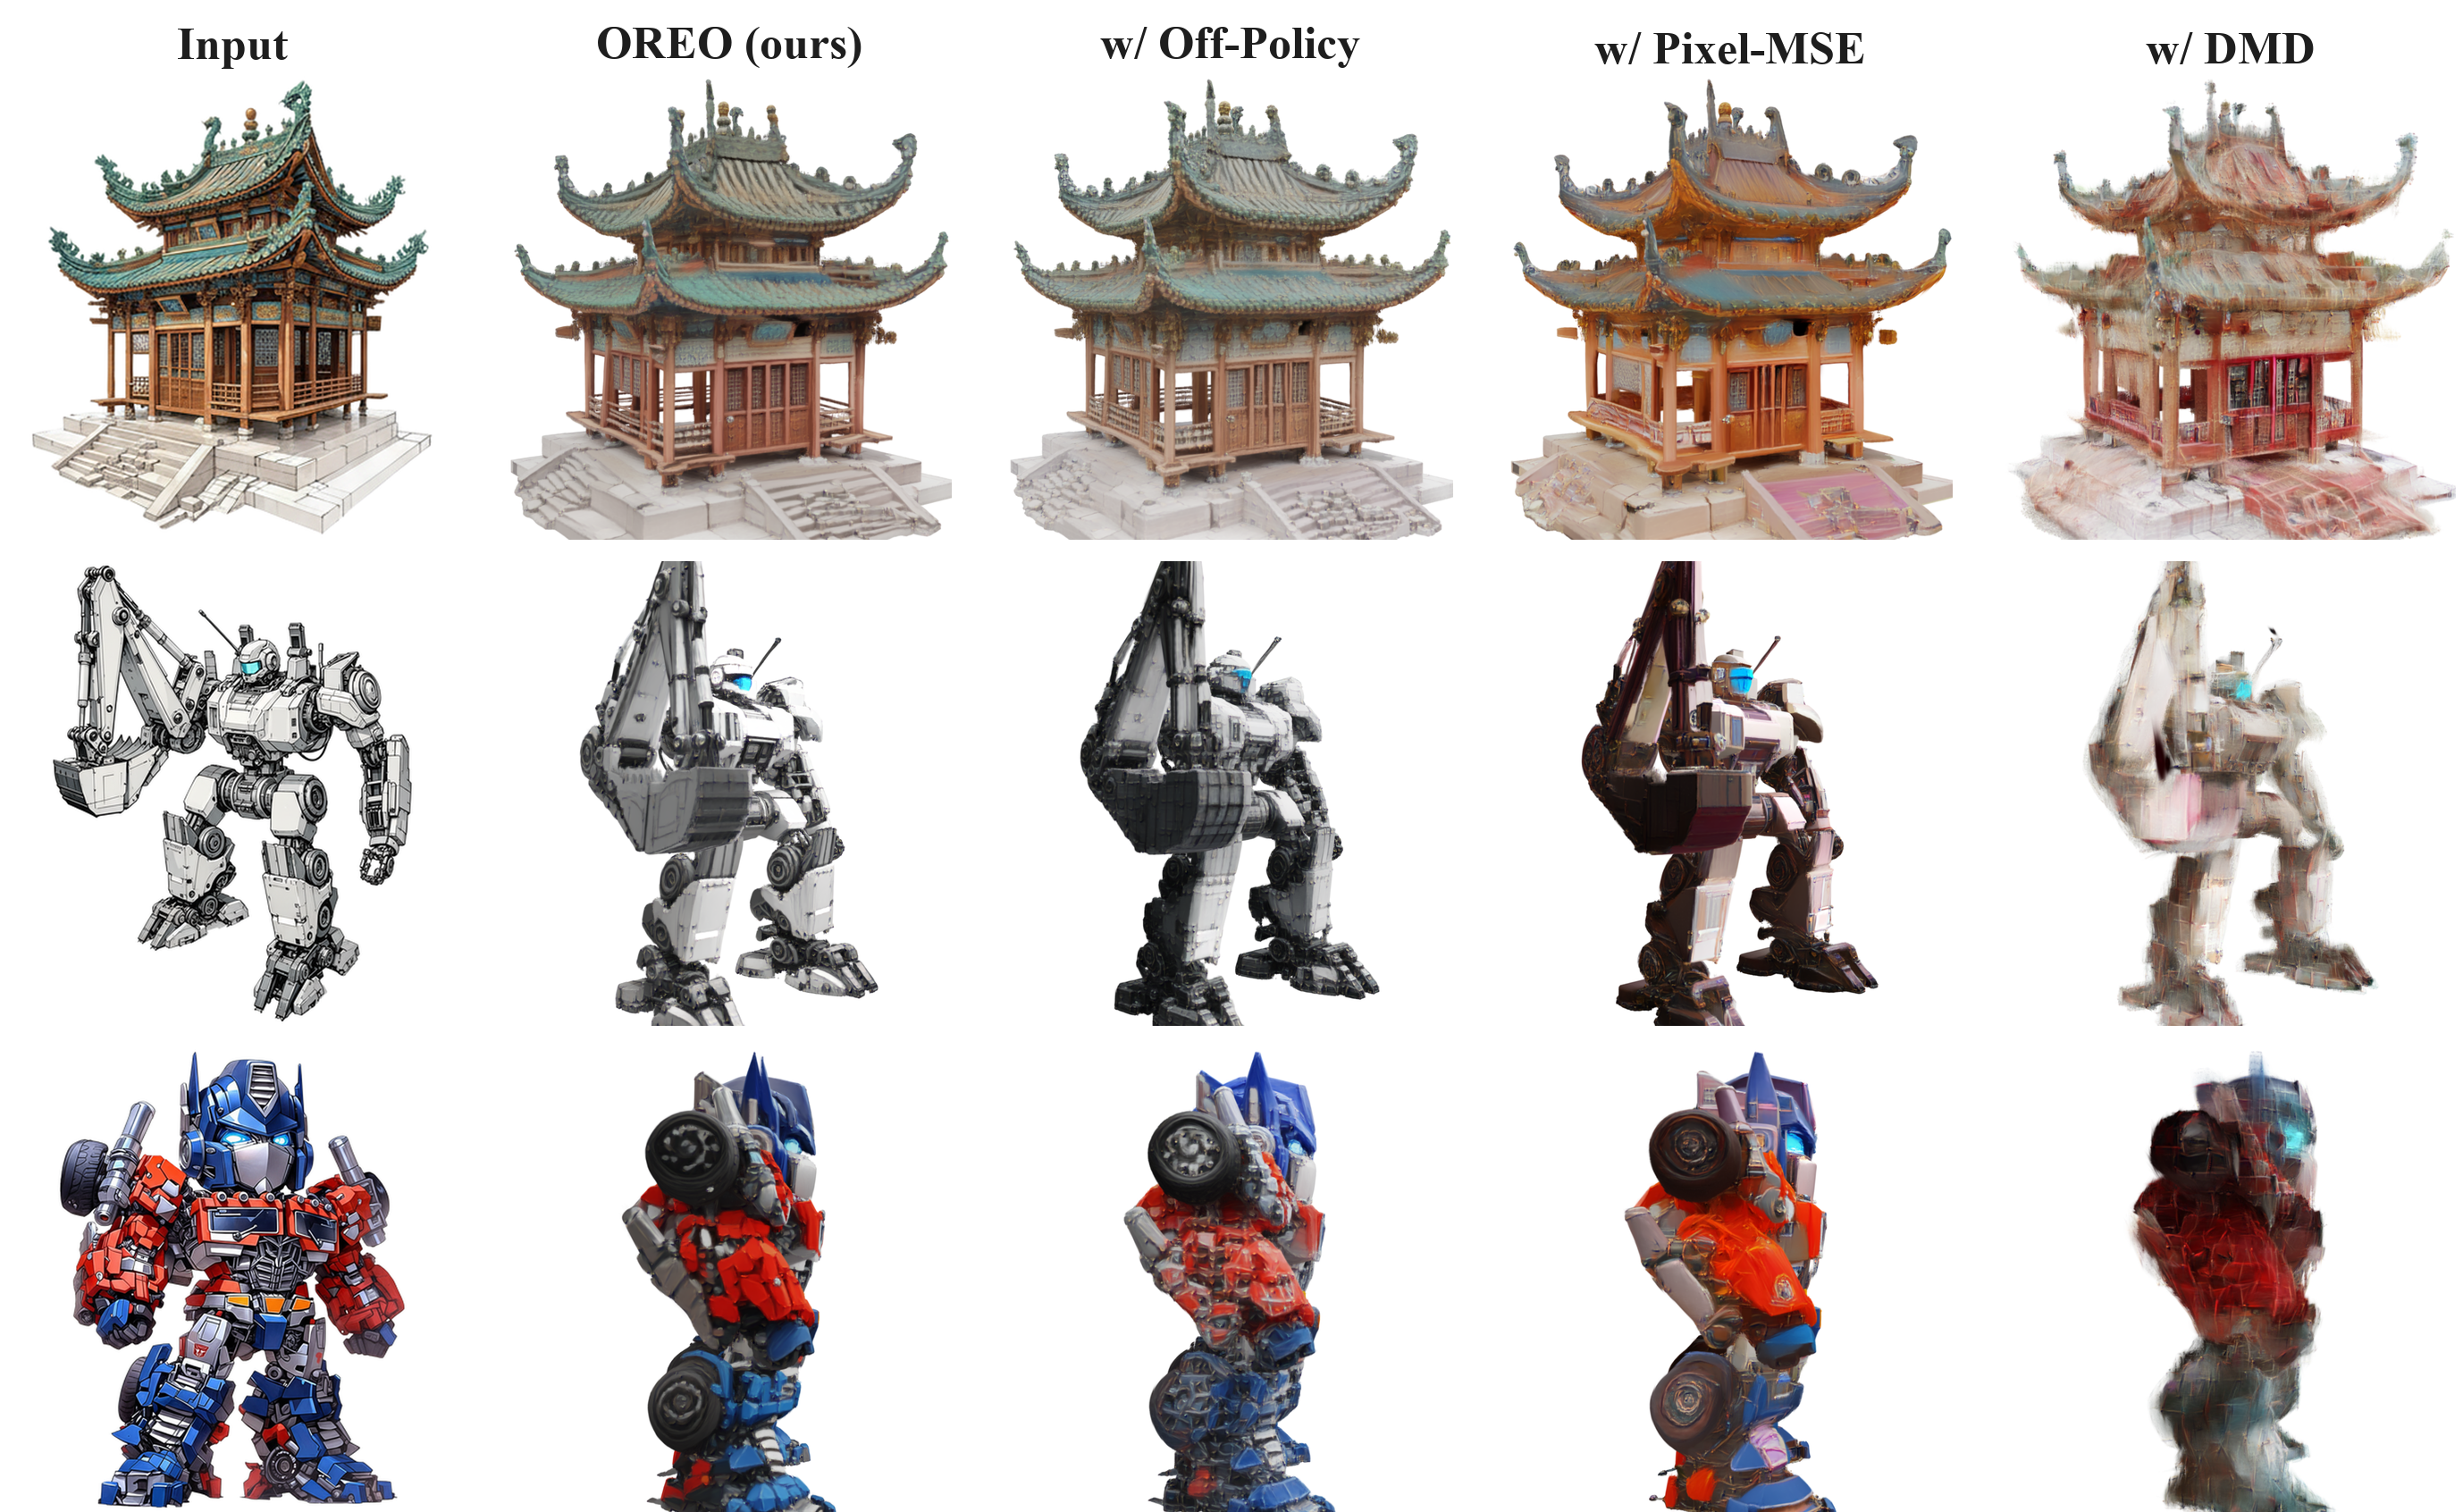
\includegraphics[width=\textwidth]{figures_final/mv_ablation_final.png}
  \caption{\textbf{Qualitative ablation of the 3D generator design choices.} We compare Full OREO against other training variants. Details are in Sec.~\ref{sec:exp_ablation}.}
  \label{fig:ablation_overview}
\end{figure*}

\begin{table}[!tbp]
  \centering
  \caption{\textbf{Ablation on the design choices of the 3D generator.} We report CLIP and DINO similarity to the reference $x^{\texttt{ref}}$ on the Conceptual Design Dataset. Details are in Sec.~\ref{sec:exp_ablation}.}
  \label{tab:ablation_quantitative}
  \begin{tabular}{@{}lcc@{}}
    \toprule
    Method / Variant & CLIP Sim. $\uparrow$ & DINO Sim. $\uparrow$ \\
    \midrule
    Pretrained Trellis & 0.7613 & 0.7916 \\
    \midrule
    \textbf{Full OREO (Ours)} & \textbf{0.7834} & \textbf{0.8065} \\
    w/ Pixel-MSE Supervision & 0.6617 & 0.6982 \\
    w/ Off-policy Rollout & 0.7279 & 0.7613 \\
    w/ DMD (Score Distillation) & 0.5393 & 0.5486 \\
    \bottomrule
  \end{tabular}
\end{table}

\textbf{Degradation under Off-policy Rollout.} Freezing the rollout to $z_0=G_{\theta_{pre}}(x^{\texttt{ref}})$ decouples the anchor from the training generator's own trajectory. Training itself remains stable, and the geometric structure is largely preserved as shown in Fig.~\ref{fig:ablation_overview}, but colors desaturate and fine-grained textures are progressively smoothed out. For example, the multi-color glazed roof in row~1 loses its saturation, and the mecha in row~3 fades into a muted red-blue palette. Quantitatively, CLIP and DINO similarity drop by $0.0555$ and $0.0452$ relative to Full OREO, and both metrics fall below the pretrained baseline.


\textbf{Attenuation of Gradient through Differentiable Rendering.} Replacing the latent contrastive loss with a pixel-space regression $\|x^{\texttt{src}}-x^{\texttt{tgt}}\|^2$ forces the gradient back through the frozen decoder $\mathcal{D}$ and renderer $\mathcal{P}$ before reaching $v_\theta$. Training does not diverge, but the attenuated gradient can no longer drive fidelity improvement, and the outputs drift toward a texture-averaged, color-shifted solution. The roof in row~1 turns uniformly beige and the excavator robot in row~2 fades into washed-out white. CLIP and DINO similarity fall to $0.6617$/$0.6982$, well below the pretrained baseline, as shown in Fig.~\ref{fig:ablation_overview}.


\textbf{Necessity of Reinforced Editing.} Rather than construct an explicit pseudo-GT, DMD supplies the training generator with a single-step score-distillation gradient obtained from the frozen 2D editor. Without a multi-step edited target, the gradient captures only a local view of the 2D prior at one noise scale, and the accumulated update over training is high-variance and directionally inconsistent. Fig.~\ref{fig:ablation_overview} shows the resulting outputs suffer from severe geometric distortion and color collapse, e.g., the mecha in row~3 loses its structural coherence entirely. CLIP and DINO similarity collapse to $0.5393$/$0.5486$, the worst among all variants, confirming that a coherent multi-step target from RE cannot be replaced by an implicit gradient signal.

\section{Conclusion}
This paper proposes \textbf{OREO}, a fidelity alignment framework for 3D generation.
Addressing the lack of visual realism in existing 3D models, we introduce an on-the-fly optimization loop that leverages 2D diffusion priors.
At its core, we propose Reinforced Editing to generate structure-preserving pseudo-GTs, which serve as dynamic supervision targets.
Experimental results demonstrate that OREO effectively enhances the visual fidelity and texture details of 3D generators while maintaining geometric integrity, offering a scalable solution to bridge the gap between 3D geometry and 2D visual realism. Limitations are provided in the \emph{Supp.\ Material}.

\textbf{Future Work.} Although OREO performs well, there is still room for further exploration. First, the current FlowEdit process has high inference costs; future work could explore more efficient distillation strategies (e.g., one-step editing). Second, we will attempt to extend OREO to more complex scene generation tasks, utilizing panoramic editing models to optimize large-scale 3D environments. Finally, combining with Large Multimodal Models (LMM) for more fine-grained interactive editing is also an exciting direction.

\clearpage

\bibliographystyle{splncs04}
\bibliography{main}

\end{document}
